\documentclass[]{article}
\usepackage[T1]{fontenc}
\usepackage{lmodern}
\usepackage{amssymb,amsmath}
\usepackage{ifxetex,ifluatex}
\usepackage{fixltx2e} % provides \textsubscript
% use upquote if available, for straight quotes in verbatim environments
\IfFileExists{upquote.sty}{\usepackage{upquote}}{}
\ifnum 0\ifxetex 1\fi\ifluatex 1\fi=0 % if pdftex
  \usepackage[utf8]{inputenc}
\else % if luatex or xelatex
  \ifxetex
    \usepackage{mathspec}
    \usepackage{xltxtra,xunicode}
  \else
    \usepackage{fontspec}
  \fi
  \defaultfontfeatures{Mapping=tex-text,Scale=MatchLowercase}
  \newcommand{\euro}{€}
\fi
% use microtype if available
\IfFileExists{microtype.sty}{\usepackage{microtype}}{}
\usepackage[margin=1in]{geometry}
\usepackage{color}
\usepackage{fancyvrb}
\newcommand{\VerbBar}{|}
\newcommand{\VERB}{\Verb[commandchars=\\\{\}]}
\DefineVerbatimEnvironment{Highlighting}{Verbatim}{commandchars=\\\{\}}
% Add ',fontsize=\small' for more characters per line
\usepackage{framed}
\definecolor{shadecolor}{RGB}{248,248,248}
\newenvironment{Shaded}{\begin{snugshade}}{\end{snugshade}}
\newcommand{\KeywordTok}[1]{\textcolor[rgb]{0.13,0.29,0.53}{\textbf{{#1}}}}
\newcommand{\DataTypeTok}[1]{\textcolor[rgb]{0.13,0.29,0.53}{{#1}}}
\newcommand{\DecValTok}[1]{\textcolor[rgb]{0.00,0.00,0.81}{{#1}}}
\newcommand{\BaseNTok}[1]{\textcolor[rgb]{0.00,0.00,0.81}{{#1}}}
\newcommand{\FloatTok}[1]{\textcolor[rgb]{0.00,0.00,0.81}{{#1}}}
\newcommand{\CharTok}[1]{\textcolor[rgb]{0.31,0.60,0.02}{{#1}}}
\newcommand{\StringTok}[1]{\textcolor[rgb]{0.31,0.60,0.02}{{#1}}}
\newcommand{\CommentTok}[1]{\textcolor[rgb]{0.56,0.35,0.01}{\textit{{#1}}}}
\newcommand{\OtherTok}[1]{\textcolor[rgb]{0.56,0.35,0.01}{{#1}}}
\newcommand{\AlertTok}[1]{\textcolor[rgb]{0.94,0.16,0.16}{{#1}}}
\newcommand{\FunctionTok}[1]{\textcolor[rgb]{0.00,0.00,0.00}{{#1}}}
\newcommand{\RegionMarkerTok}[1]{{#1}}
\newcommand{\ErrorTok}[1]{\textbf{{#1}}}
\newcommand{\NormalTok}[1]{{#1}}
\usepackage{graphicx}
% Redefine \includegraphics so that, unless explicit options are
% given, the image width will not exceed the width of the page.
% Images get their normal width if they fit onto the page, but
% are scaled down if they would overflow the margins.
\makeatletter
\def\ScaleIfNeeded{%
  \ifdim\Gin@nat@width>\linewidth
    \linewidth
  \else
    \Gin@nat@width
  \fi
}
\makeatother
\let\Oldincludegraphics\includegraphics
{%
 \catcode`\@=11\relax%
 \gdef\includegraphics{\@ifnextchar[{\Oldincludegraphics}{\Oldincludegraphics[width=\ScaleIfNeeded]}}%
}%
\ifxetex
  \usepackage[setpagesize=false, % page size defined by xetex
              unicode=false, % unicode breaks when used with xetex
              xetex]{hyperref}
\else
  \usepackage[unicode=true]{hyperref}
\fi
\hypersetup{breaklinks=true,
            bookmarks=true,
            pdfauthor={},
            pdftitle={},
            colorlinks=true,
            citecolor=blue,
            urlcolor=blue,
            linkcolor=magenta,
            pdfborder={0 0 0}}
\urlstyle{same}  % don't use monospace font for urls
\setlength{\parindent}{0pt}
\setlength{\parskip}{6pt plus 2pt minus 1pt}
\setlength{\emergencystretch}{3em}  % prevent overfull lines
\setcounter{secnumdepth}{0}

\author{}
\date{}

\begin{document}

\begin{center}
\normalsize
\end{center}


\section{The Effect of Transmission on Fuel
Economy}\label{the-effect-of-transmission-on-fuel-economy}

\subsection{Executive Summary}\label{executive-summary}

The purpose of this analysis is to quantify the relationship between
vehicle transmission and fuel economy, measured in miles per gallon
(mpg). The data we use is taken from the \texttt{mtcars} dataset
included in the R programming language . This data is taken from the
1974 Motor Trend magazine, and details 11 aspects of motor vehicle
design and performance. We find that on average, cars with manual
transmissions are more fuel efficient than those with automatic
transmissions by 2.08 miles per gallon. This effect, however, is not
statistically significant after adjusting for variations in weight and
horsepower.

\section{Analysis}\label{analysis}

This analysis requires the \texttt{ggplot2} and \texttt{GGally} graphics
packages, and the \texttt{mtcars} dataset. In Figure 1, we create a
matrix plot of the columns of mtcars to see what relationships there are
between the variables. Figure 2 is a boxplot comparing fuel economy
between automatic and manual transmission cars.

We find many relationships between various columms. This can be
problematic for linear regression; omitting interaction terms can make
models less accurate, but including these terms makes models much harder
to interpret. We will fit a linear model in a stepwise fashion without
interaction terms, starting with transmission type. To limit the effect
of the corelation between variables, we will limit our model to 3
predictors.

First, we create the one-predictor model based on transmission type.

\begin{Shaded}
\begin{Highlighting}[]
\NormalTok{mpg_am <-}\StringTok{ }\KeywordTok{lm}\NormalTok{(mpg ~}\StringTok{ }\NormalTok{am, }\DataTypeTok{data=}\NormalTok{mtcars)}
\KeywordTok{summary}\NormalTok{(mpg_am)[}\KeywordTok{c}\NormalTok{(}\StringTok{"coefficients"}\NormalTok{,}\StringTok{"r.squared"}\NormalTok{)]}
\end{Highlighting}
\end{Shaded}

\begin{verbatim}
## $coefficients
##             Estimate Std. Error t value  Pr(>|t|)
## (Intercept)   17.147      1.125  15.247 1.134e-15
## am             7.245      1.764   4.106 2.850e-04
## 
## $r.squared
## [1] 0.3598
\end{verbatim}

As expected, our model does not do a great job of explaining the
variance in the data set; the R squared is only 0.338.

The next predictor we add is the one which improves the R squared
statistic the most; to find this predictor, we caclulate the linear
regression for each remaining column and compare the R squared.

\begin{Shaded}
\begin{Highlighting}[]
\NormalTok{variablesLeft <-}\StringTok{ }\KeywordTok{setdiff}\NormalTok{(}\KeywordTok{names}\NormalTok{(mtcars), }\KeywordTok{c}\NormalTok{(}\StringTok{"mpg"}\NormalTok{, }\StringTok{"am"}\NormalTok{))}
\NormalTok{models1 <-}\StringTok{ }\KeywordTok{lapply}\NormalTok{(variablesLeft, }\DataTypeTok{FUN=}\NormalTok{function(x) \{}
    \NormalTok{form <-}\StringTok{ }\KeywordTok{paste0}\NormalTok{(}\StringTok{"mpg ~ am + "}\NormalTok{, x)}
    \KeywordTok{lm}\NormalTok{(form, }\DataTypeTok{data=}\NormalTok{mtcars)}
\NormalTok{\})}
\NormalTok{results <-}\StringTok{ }\KeywordTok{cbind}\NormalTok{(}\DataTypeTok{column=}\NormalTok{variablesLeft, }
                 \DataTypeTok{adj.r.squared=}\KeywordTok{sapply}\NormalTok{(models1, }
                                      \DataTypeTok{FUN=}\NormalTok{function(x) }\KeywordTok{summary}\NormalTok{(x)$adj.r.squared))}
\NormalTok{results[}\KeywordTok{order}\NormalTok{(results[,}\DecValTok{2}\NormalTok{], }\DataTypeTok{decreasing=}\OtherTok{TRUE}\NormalTok{)[}\DecValTok{1}\NormalTok{],]}
\end{Highlighting}
\end{Shaded}

\begin{verbatim}
##              column       adj.r.squared 
##                "hp" "0.767002539013904"
\end{verbatim}

\begin{Shaded}
\begin{Highlighting}[]
\KeywordTok{summary}\NormalTok{(models1[[}\DecValTok{3}\NormalTok{]])[}\KeywordTok{c}\NormalTok{(}\StringTok{"coefficients"}\NormalTok{,}\StringTok{"r.squared"}\NormalTok{)]}
\end{Highlighting}
\end{Shaded}

\begin{verbatim}
## $coefficients
##             Estimate Std. Error t value  Pr(>|t|)
## (Intercept) 26.58491   1.425094  18.655 1.074e-17
## am           5.27709   1.079541   4.888 3.460e-05
## hp          -0.05889   0.007857  -7.495 2.920e-08
## 
## $r.squared
## [1] 0.782
\end{verbatim}

We find that the model evaluating horsepower has the highest R squared
statistic. We repeat the process to find our last predictor to add to
the model.

\begin{Shaded}
\begin{Highlighting}[]
\NormalTok{variablesLeft <-}\StringTok{ }\KeywordTok{setdiff}\NormalTok{(variablesLeft, }\StringTok{"hp"}\NormalTok{)}
\NormalTok{models2 <-}\StringTok{ }\KeywordTok{lapply}\NormalTok{(variablesLeft, }\DataTypeTok{FUN=}\NormalTok{function(x) \{}
    \NormalTok{form <-}\StringTok{ }\KeywordTok{paste0}\NormalTok{(}\StringTok{"mpg ~ am + hp + "}\NormalTok{, x)}
    \KeywordTok{lm}\NormalTok{(form, }\DataTypeTok{data=}\NormalTok{mtcars)}
\NormalTok{\})}

\NormalTok{results <-}\StringTok{ }\KeywordTok{cbind}\NormalTok{(}\DataTypeTok{column=}\NormalTok{variablesLeft, }
                 \DataTypeTok{adj.r.squared=}\KeywordTok{sapply}\NormalTok{(models2, }
                                      \DataTypeTok{FUN=}\NormalTok{function(x) }\KeywordTok{summary}\NormalTok{(x)$adj.r.squared))}
\NormalTok{results[}\KeywordTok{order}\NormalTok{(results[,}\DecValTok{2}\NormalTok{], }\DataTypeTok{decreasing=}\OtherTok{TRUE}\NormalTok{)[}\DecValTok{1}\NormalTok{],]}
\end{Highlighting}
\end{Shaded}

\begin{verbatim}
##              column       adj.r.squared 
##                "wt" "0.822735694896529"
\end{verbatim}

\begin{Shaded}
\begin{Highlighting}[]
\KeywordTok{summary}\NormalTok{(models2[[}\DecValTok{4}\NormalTok{]])[}\KeywordTok{c}\NormalTok{(}\StringTok{"coefficients"}\NormalTok{,}\StringTok{"r.squared"}\NormalTok{)]}
\end{Highlighting}
\end{Shaded}

\begin{verbatim}
## $coefficients
##             Estimate Std. Error t value  Pr(>|t|)
## (Intercept) 34.00288   2.642659  12.867 2.824e-13
## am           2.08371   1.376420   1.514 1.413e-01
## hp          -0.03748   0.009605  -3.902 5.464e-04
## wt          -2.87858   0.904971  -3.181 3.574e-03
## 
## $r.squared
## [1] 0.8399
\end{verbatim}

We find that weight explains the most variance in the rest of the data.
Holding these two covariates constant, we find that the difference
between manual and automatic transmission fuel economy is 2.08, but is
not significant. Looking at the Residuals plot in Figure 4, we see that
there is a distinct U shape in the plot; this is not unexpected, as we
intentionally disregarded the effect of interactions between the
variables and limited the number of predictors in the model.
Incorporating interaction terms would likely improve the fit of the
model and reduce the pattern in this residuals plot.

The major weakness of this analysis is that by ignoring interaction
terms, we sacrifice power in order to make the interpretation of the
model easier. As such, our conclusion of a lack of relation between mpg
and transmission type must be taken cautiously. A study with a larger
sample size that considers the interaction between the variables may
yield better results.

\section{Appendix: Figures}\label{appendix-figures}

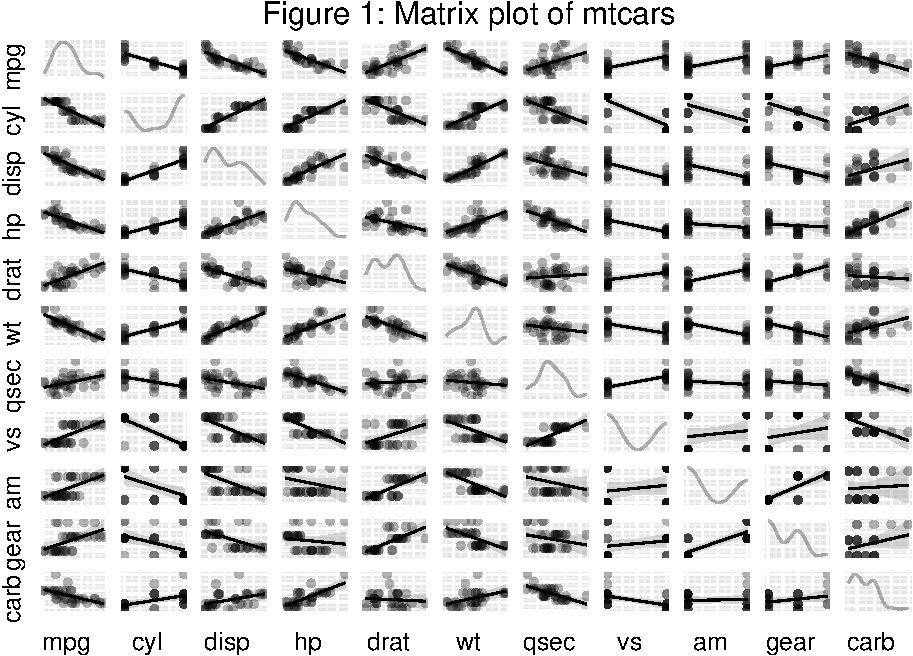
\includegraphics{./analysis_files/figure-latex/Figures1.pdf}
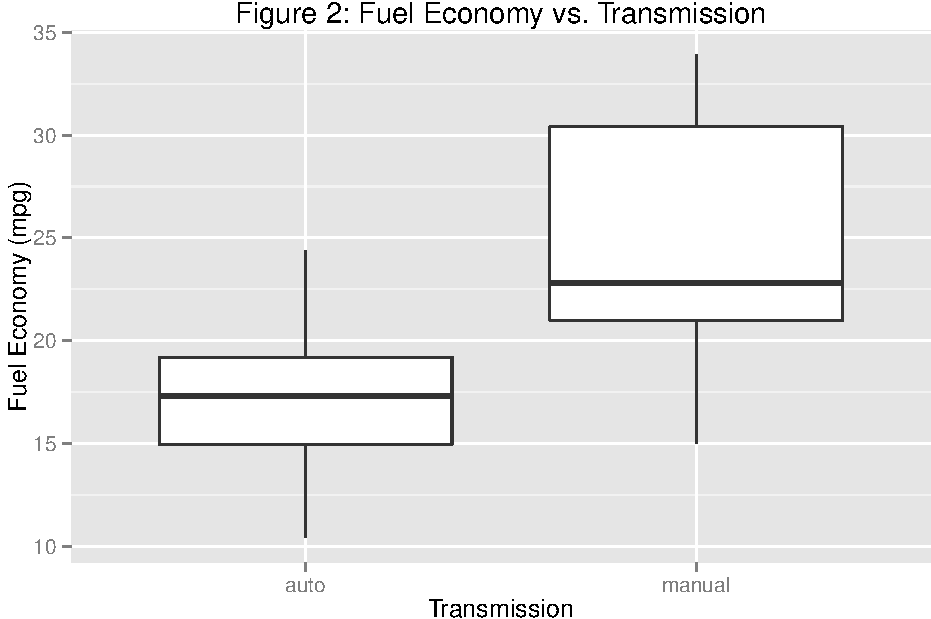
\includegraphics{./analysis_files/figure-latex/Figures2.pdf}
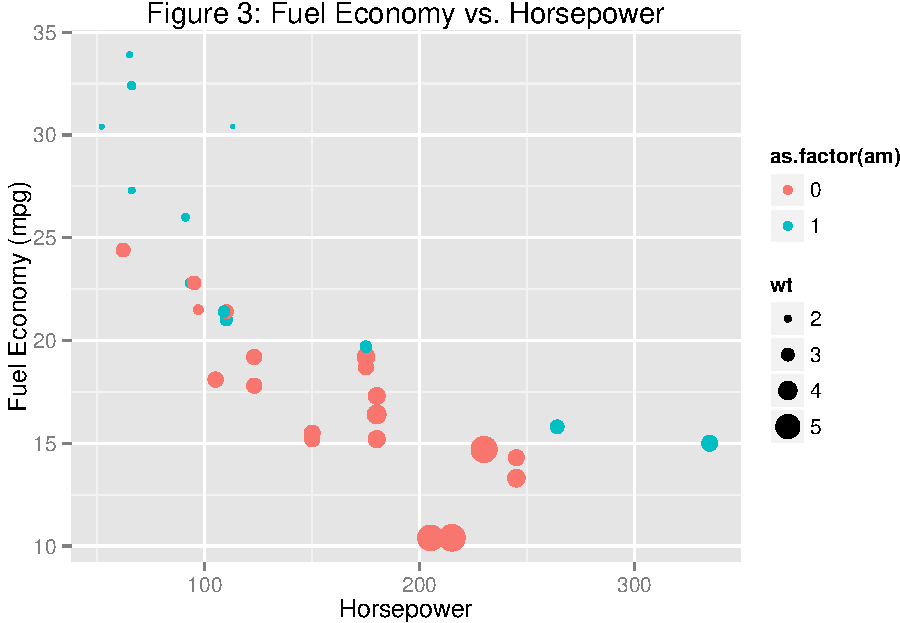
\includegraphics{./analysis_files/figure-latex/Figures3.pdf}
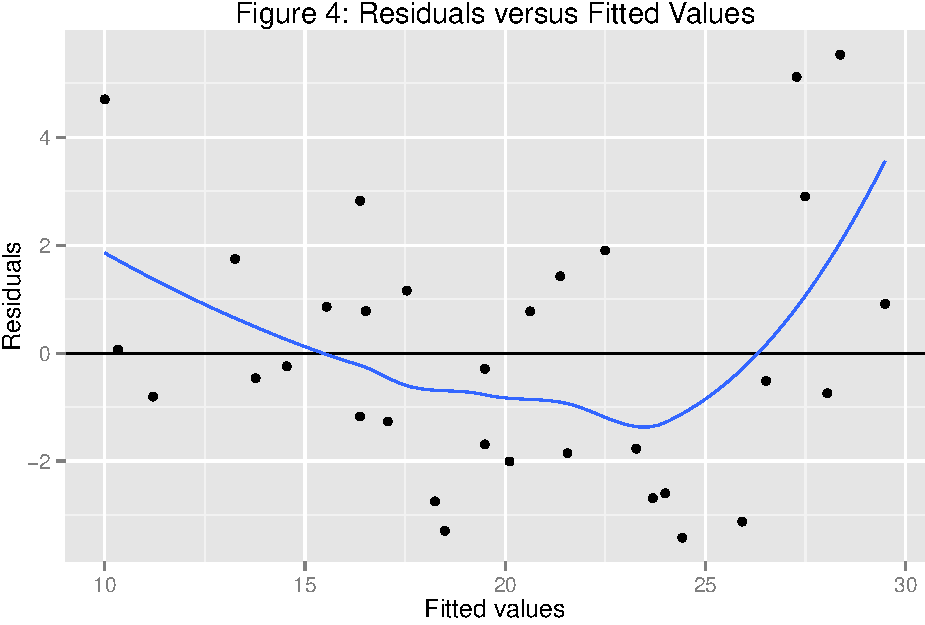
\includegraphics{./analysis_files/figure-latex/Figures4.pdf}

\end{document}
